\section{Redcuing security to safety}

% Explain the paper, in your own words. Don't go into as many details as the
% original text, but the person reading your review should have a general
% understanding of the paper's results and how those results can be obtained.
% The structure and content of this section of course heavily depends on the
% paper itself. Don't hesitate to split it in multiple sections or subsections,
% for example: \subsection{An algorithm for whatever problem we try to solve} If
% your paper contains theorems, sketch the proofs of important theorems.

% \subsection{Benchmarks} If it contains benchmarks, show the key scores or
% results.

% You can follow the structure of the paper you're reviewing, but write with
% your own words.

% \subsection{Reducing security to safety}

At the interface of any security-sensitive function call, there usually exists a
\emph{contract} that describes which inputs or outpus are deemed public (i.e.,
known to attackers) and which ones are private (i.e., to protect). A leak should
never reveal anyting about the private inputs and outputs (but publics ones 
can be leaked).
If we denote a program as $p$ (with the usual definition of a prgram being a
sequence of statements or programs) with a corresponding state $s$ (which
is mapping from variables to values) then at each step of execution, from
state $s$ executing program/statement $p$ we can define leakage $L(.)$ as follows:

\begin{equation}
    \begin{split}
    L(\langle s, \text{\texttt{if}}~e~\text{\texttt{then}}~p_1~\text{\texttt{else}}~p_2 \rangle) = & s(e) \\
    L(\langle s, \text{\texttt{while}}~e~\text{\texttt{do}}~p \rangle) = & s(e) \\
    L(\langle s, x_0[e_0] = e \rangle) = & s(e_0)s(e_1)...s(e_n)
    \end{split}
\end{equation}

The first two leakage sources correspond to leakage from control flow while the
latter is leakage from memory access. Note that in the third leakage source,
a memory leak $s(e_0)$ corresponds to leakage from the right-hand-side indexer
expression and $s(e_1)$ to $s(e_n)$ possible indexer expression in expression
$e$. We can also extend the leakage sources to comprise machine operations that
have operand-dependent execution latency (i.e., division in x86).

Using the leakage rules above, we can reduce proving constant-time security to
execution safety (i.e., termination without any failed assertions) by building a
\emph{self-product} in which two abstract execution take place back to back,
only differing in the value of private inputs and outputs.
Figure~\ref{fig:rules} shows how a program product can be constructed where 
$\hat{p}$ is the program $p$ with all variables renamed.

\begin{figure}[h]
    \centering
    \subfigure[Program product construction rules]{
        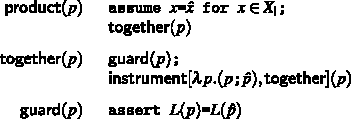
\includegraphics[width=0.45\textwidth]{./figs/fig_7.pdf}
    }\label{fig:fig_7}
    \subfigure[Instrumentation rules] {
        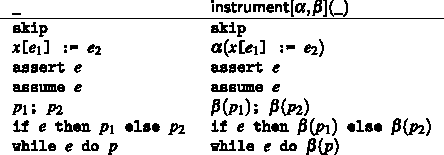
\includegraphics[width=0.45\textwidth]{./figs/fig_8.pdf}
    }\label{fig:fig_8}
    \caption{Program product}
    \label{fig:rules}
\end{figure}


The essence of the transformation is the instrumentation, which reduces 
constant-time security to assertion safety. \figref{fig:example_prod} shows 
the product of the sub-array copy program. Notice how  the program is instrumented
with assertion to ensure leakage remains the same at every step of execution.
In this example, the private inputs \texttt{l\_idx} and its renaming are not
assumed to be equal, therefore the assetion on line 8 fails and the program 
is proved to be unsafe and hence it follows that the program is not constant-time
secure.

\begin{figure}[h]
    \begin{lstlisting}[language=MySketch]
        assume in = $\hat{\texttt{in}}$;
        assume out = $\hat{\texttt{out}}$;
        assume len = $\hat{\texttt{len}}$;
        assume sub_len = $\hat{\texttt{sub\_len}}$;
        i = 0; $\hat{\texttt{i}}$ = 0; j = 0; $\hat{\texttt{j}}$ = 0;
        assert (i < len) = ($\hat{\texttt{i}}$ < $\hat{\texttt{len}}$); // trivial
        while (i < len) do:
          assert ((i $\geq$ l_idx) && (i < l_idx + sub_len)) = (($\hat{\texttt{i}}$ $\geq$ _l_idx) && ($\hat{\texttt{i}}$ < _l_idx + $\hat{\texttt{sub\_len}}$) // fails;
          if ((i $\geq$ l_idx) && (i < l_idx + sub_len)) then
              /// the rest of the program does not matter
              assert i = $\hat{\texttt{i}}$ && j = $\hat{\texttt{j}}$
              out[j] = in[i]; $\hat{\texttt{out}}$[$\hat{\texttt{j}}$] = $\hat{\texttt{in}}$[_i];
              j = j + 1; $\hat{\texttt{j}}$ = $\hat{\texttt{j}}$ + 1;
          i = i + 1; $\hat{\texttt{i}}$ = $\hat{\texttt{i}}$ + 1;
      \end{lstlisting}
      \caption{example program product of the sub-array copy program.}
      \label{fig:example_prod}
\end{figure}

